% Body of the paper. Included from main.tex.

\section{Introduction}

Physics-informed neural networks \citep{raissi2019pinn} solve a PDE by
minimising its residual at collocation points, and a large literature now
supplies training machinery to make that minimisation work: causal time
weighting \citep{wang2022causal}, gradient-norm balancing of the loss terms
\citep{wang2021gradientflow,wang2023expert}, residual-based attention
\citep{anagnostopoulos2024rba}, Fourier feature embeddings
\citep{tancik2020fourier,wang2021fourier}, residual-adaptive architectures
\citep{wang2024piratenet}, Kolmogorov--Arnold layers
\citep{liu2024kan,bozorgasl2024wavkan,shukla2024pikan}, and second-order
optimisers \citep{vyas2024soap,wang2025soappinn}. Each is reported to improve
on a baseline PINN. What is much less often reported is how the resulting
system compares to a classical discretisation of the same equation, run on the
same problem, and measured with the same metric.

This paper makes that comparison on one deliberately modest problem: the 1D
elastic wave equation in a heterogeneous medium,
\begin{equation}
\rho(x)\, u_{tt} \;=\; \partial_x\!\left[E(x)\, u_x\right],
\qquad x \in [x_{\min}, x_{\max}],\ t \in [0,1],
\label{eq:wave}
\end{equation}
with a Gaussian-derivative initial pulse, zero initial velocity, and
first-order radiation conditions at both ends. The problem is small enough
that a classical solver is essentially free, which is exactly what makes it a
useful control: any claim that a PINN is doing something valuable has to be
made against a baseline whose accuracy and cost are both known.

Running that control produced a result we were not looking for. Two of the
adaptive schemes above --- causal time weighting and GradNorm balancing ---
turn out to \emph{cost} an order of magnitude of accuracy on this problem when
run as specified. Switching both off improves relative $L^2$ by
$\AblMinGain$--$\AblMaxGain\times$. Neither is misbehaving: both do exactly
what their specification says, and what the specification does here is leave
most of the time domain untrained and the PDE residual weighted a thousand
times below the boundary term. This is invisible if a run is reported by its
final error alone, and obvious from diagnostics the methods already compute.

\paragraph{Contributions.}
\begin{enumerate}\itemsep2pt
\item \textbf{A characterised classical baseline.} We implement three
  discretisations of \eqref{eq:wave} --- second-order finite differences in
  flux form, linear finite elements with a lumped mass matrix, and Chebyshev
  collocation on the velocity--stress system --- and measure error against a
  self-converged spectral solution. The spectral solver reaches
  $\ChebHomogeneousErr\%$ relative $L^2$ on the homogeneous case in
  \SI{\ChebHomogeneousSecs}{\second}; the two second-order schemes are
  indistinguishable from each other and \emph{plateau} at $\FDFloor\%$.
\item \textbf{An accuracy floor in the reference itself.} That plateau is not
  the interior stencil. It is the first-order Mur absorbing boundary
  \citep{mur1981abc}: refining from 1\,600 to 6\,400 cells moves the error by
  less than $0.1\%$ of its own value. Every PINN number in this literature that
  is scored against a finite-difference reference inherits this floor, and it
  is worth knowing where it sits before reading a small error as a small error.
\item \textbf{The published training recipe, run end to end.} We evaluate seven
  coordinate-network architectures on three material profiles under two initial
  condition treatments, with the causal/GradNorm recipe as specified, plus
  SOAP and residual-based-attention arms.
\item \textbf{Both adaptive weighting schemes make things worse.} Switching
  causal weighting and GradNorm off --- pinning
  $w_{\mathrm{pde}} = w_{\mathrm{bc}} = w_{\mathrm{ic}} = 1$ and weighting every
  time slab equally --- improves relative $L^2$ in
  $\AblWins$ of $\AblPairCount$ architecture--material cells, which is all of
  them, by $\AblMinGain$--$\AblMaxGain\times$ (median $\AblMedianGain\times$),
  from $\PinnRecipeBestErr\%$ to $\AblBestErr\%$ for the best architecture.
  This is the paper's main result and it was not what we set out to look for.
\item \textbf{A mechanism, not a mystery.} The causal frontier advances two
  slabs of sixteen and stops, so most of the time domain carries weight exactly
  zero for all $24\,000$ Adam steps including the continuation budget; GradNorm
  independently settles at $w_{\mathrm{pde}} \approx 0.001$ against
  $w_{\mathrm{bc}} \approx 1.999$. Both are visible in diagnostics these methods
  already compute.
\end{enumerate}

\section{Problem, materials, and what ``exact'' means here}
\label{sec:problem}

\paragraph{Equation and non-dimensionalisation.}
We use the conservative form \eqref{eq:wave} throughout. Expanding it gives
$\rho u_{tt} = E u_{xx} + E_x u_x$, so the frequently used
$u_{tt} = c(x)^2 u_{xx}$ drops the $E_x u_x$ term --- precisely the term that
sets reflection and transmission amplitudes at a material interface. Each
material is non-dimensionalised by a reference stiffness $E_{\mathrm{ref}}$ and
density $\rho_{\mathrm{ref}}$ and a half-length $L_{\mathrm{ref}}$, so that
$\rho \equiv 1$, $E = O(1)$, and $x \in [-1,1]$.

\paragraph{Materials.} Three profiles of increasing difficulty, all with
$\rho \equiv 1$ so that $c(x) = \sqrt{E(x)}$:
\emph{Homogeneous} ($E \equiv 1$);
\emph{TwoLayer}, a $\tanh$-smoothed step from $E = 1$ to $E = 1.5$ at $x=0$
with interface half-width $0.02$; and
\emph{MultiLayer}, six $\tanh$-blended layers with $E$ from $1$ to $2.5$.
The interfaces are smooth but narrow: at half-width $0.02$ on a domain of
length $2$, resolving one costs roughly a hundred grid points.

\paragraph{Initial and boundary conditions.}
$u(x,0) = f(x)$ is the derivative of a Gaussian of width $\sigma_g = 0.1$,
normalised to unit peak, and $u_t(x,0)=0$. Because the initial velocity
vanishes, the pulse splits into two counter-propagating waves of roughly half
amplitude. Both boundaries carry the first-order radiation condition
$u_t \mp c\,u_x = 0$, so waves leave the domain rather than reflecting.

\paragraph{Metric.} All errors are relative $L^2$ in percent on a shared
$201 \times 101$ evaluation grid over $(x,t)$,
$100\,\lVert \hat u - u \rVert_2 / \lVert u \rVert_2$. This has a useful
calibration property: a model that predicts zero everywhere scores
approximately $100\%$, so any number near or above $100$ indicates a solution
that carries no signal.

\section{Classical baselines}
\label{sec:classical}

We implement three discretisations of \eqref{eq:wave}, all sharing the problem
above and all returning $u$ resampled onto the evaluation grid so that the
metric never depends on a solver's internal resolution.

\textbf{\texttt{fd2}} is the explicit second-order leapfrog scheme in flux
form, with harmonic-mean interface stiffness
$E_{i+1/2} = 2E_iE_{i+1}/(E_i+E_{i+1})$ and Mur-discretised absorbing
boundaries $u_0^{n+1} = u_1^{n} + \beta(u_1^{n+1} - u_0^{n})$,
$\beta = (c\,\Delta t - \Delta x)/(c\,\Delta t + \Delta x)$. This is the
reference solver the PINN runs are scored against.

\textbf{\texttt{fem\_p1}} uses linear elements with two-point Gauss evaluation
of the element coefficients, a lumped mass matrix, and explicit central
differences. The radiation condition appears in the weak form as a boundary
$\rho c$ dashpot, so it needs no special discretisation.

\textbf{\texttt{cheb}} collocates the velocity--stress system
$\rho v_t = \partial_x \sigma$, $\sigma_t = E\, \partial_x v$, $u_t = v$ on
Chebyshev--Gauss--Lobatto nodes and integrates with RK4. Splitting into first
order is what makes the boundary tractable: the radiation condition becomes
``the incoming Riemann invariant is zero'', imposed as a projection at every
Runge--Kutta stage. The second-order form has no stable second-order absorbing
update --- advancing $u$ at the end nodes from $u^{n-1}$ decouples them from
the interior and the corner modes grow without bound, which is what we observed
before switching formulations.

\paragraph{Ground truth.} We take a converged \texttt{cheb} solution
($n = 512$) as ground truth rather than a fine finite-difference solve, for the
reason Table~\ref{tab:classical} makes plain. Its self-convergence is reported
alongside every result: on \emph{Homogeneous}, $n = 384$ and $n = 512$ differ
by $1.3\times10^{-12}$ percent.

% generated by make_tables.py -- do not edit
\begin{table}[t]
\centering
\caption{Cost of accuracy for the three classical discretisations, measured against a converged spectral solution. Each pair of columns gives the cheapest resolution on the refinement ladder that reaches the target and the wall-clock seconds it took (best of three, one CPU core). \textit{n/a} means no resolution on the ladder reaches it. \textbf{Floor} is where the method stops improving: the two second-order schemes stall at the same $0.04\%$ on all three materials, which is the first-order Mur absorbing boundary rather than the interior stencil.}
\label{tab:classical}
\small
\begin{tabular}{llrrrrrrr}
\toprule
 & & \multicolumn{2}{c}{$\leq 1\%$} & \multicolumn{2}{c}{$\leq 0.1\%$} & \multicolumn{2}{c}{$\leq 0.01\%$} & floor \\
\cmidrule(lr){3-4}\cmidrule(lr){5-6}\cmidrule(lr){7-8}\cmidrule(lr){9-9}
material & method & $n$ & s & $n$ & s & $n$ & s & \% \\
\midrule
\multirow{3}{*}{Homogeneous} & \texttt{fd2} (FD2) & 200 & 0.0020 & 800 & 0.0062 & \textit{n/a} & -- & 0.040 \\
 & \texttt{fem\_p1} (P1 FEM) & 200 & 0.0021 & 800 & 0.0070 & \textit{n/a} & -- & 0.040 \\
 & \texttt{cheb} (spectral) & 64 & 0.1303 & 64 & 0.1303 & 64 & 0.1303 & $\approx$ ref. \\
\midrule
\multirow{3}{*}{TwoLayer} & \texttt{fd2} (FD2) & 200 & 0.0022 & 800 & 0.0076 & \textit{n/a} & -- & 0.040 \\
 & \texttt{fem\_p1} (P1 FEM) & 200 & 0.0023 & 800 & 0.0081 & \textit{n/a} & -- & 0.040 \\
 & \texttt{cheb} (spectral) & 96 & 0.3154 & 128 & 0.6469 & 192 & 2.05 & 9.5e{-}4 \\
\midrule
\multirow{3}{*}{MultiLayer} & \texttt{fd2} (FD2) & 200 & 0.0022 & 800 & 0.0101 & \textit{n/a} & -- & 0.039 \\
 & \texttt{fem\_p1} (P1 FEM) & 200 & 0.0023 & 800 & 0.0106 & \textit{n/a} & -- & 0.039 \\
 & \texttt{cheb} (spectral) & 64 & 0.2167 & 128 & 0.9383 & 256 & 6.84 & 2.7e{-}3 \\
\bottomrule
\end{tabular}
\end{table}


\paragraph{The two second-order schemes are the same scheme.} \texttt{fd2} and
\texttt{fem\_p1} agree to within $2\%$ of their own error at every resolution
on every material. This is expected rather than surprising --- a lumped-mass P1
element on a uniform grid reduces to the three-point stencil --- but it is a
useful control: two independent implementations, one derived from a Taylor
expansion and one from a weak form with a different boundary treatment,
landing on the same numbers means neither carries an implementation error large
enough to matter at this scale.

\paragraph{The reference has a floor, and it is the boundary.}
Both second-order schemes stop improving at $\FDFloor\%$, and
Table~\ref{tab:reffloor} in Appendix~\ref{app:supporting} shows where: going
from $N_x = 1000$ to $N_x = 8000$ --- a $64\times$ increase in
work --- changes the error by less than $2\%$ of its own value. The floor is
identical across the three materials to three significant figures, which is
what identifies it: the interior physics differs enormously between a constant
medium and a six-layer stack, so a shared limit cannot come from the interior
stencil. It comes from the first-order Mur absorbing boundary, which admits a
small reflected wave that no amount of grid refinement removes. The spectral
solver, whose radiation condition is exact on the characteristic variables, has
no such floor and self-converges to $\RefSelfConvHomogeneous\%$.

This matters beyond the classical comparison. The PINN runs in
Section~\ref{sec:results} are scored against \texttt{fd2} at $N_x = 1000$,
which is $\FDRefErr\%$ from the true solution. That is far below any network
error we measured, so no conclusion here is threatened by it --- but it does
bound what a PINN result on this problem could ever mean, and reporting a PINN
error of $10^{-4}$ against such a reference would be reporting agreement with a
boundary artefact.

\paragraph{Cost.} Reaching $0.1\%$ costs \SI{6}{\milli\second} to
\SI{11}{\milli\second} on one CPU core for the second-order schemes, and
$0.01\%$ is unreachable for them at any resolution. The spectral solver reaches
$\ChebTwoLayerErr\%$ on \emph{TwoLayer} in \SI{\ChebTwoLayerSecs}{\second} and
$\ChebMultiLayerErr\%$ on \emph{MultiLayer} in
\SI{\ChebMultiLayerSecs}{\second}. On \emph{Homogeneous} it reaches
$\ChebHomogeneousErr\%$ in \SI{\ChebHomogeneousSecs}{\second} at $n = \ChebHomogeneousN$.
These are the numbers a network has to be compared against.

\section{Coordinate networks}
\label{sec:pinn}

\paragraph{Architectures.} Seven, spanning the two families the PINN
literature has converged on. \emph{VanillaPINN} is a $\tanh$ MLP.
\emph{FourierFeaturePINN} prepends a trainable random Fourier embedding
\citep{tancik2020fourier,wang2021fourier}. \emph{PirateNet} uses a fixed
Fourier embedding, random weight factorisation, and residual blocks whose gate
is initialised to zero \citep{wang2024piratenet}. On the
Kolmogorov--Arnold side \citep{liu2024kan}: \emph{KAN} places a B-spline on
each edge together with a SiLU base branch; \emph{WavKAN} replaces the spline
with a wavelet \citep{bozorgasl2024wavkan}; \emph{ChebyshevKAN} is the cPIKAN
basis, a $\tanh$-squashed Chebyshev recurrence per edge
\citep{shukla2024pikan}; and \emph{FourierWavKAN} feeds a random Fourier
embedding into a WavKAN trunk.

\paragraph{Loss.} Writing $r = \rho u_{tt} - \partial_x[E u_x]$ for the
residual, the objective is
\begin{equation}
\mathcal{L} = w_{\mathrm{pde}}\,\mathcal{L}_{\mathrm{pde}}
            + w_{\mathrm{bc}}\,\mathcal{L}_{\mathrm{bc}}
            + w_{\mathrm{ic}}\,\mathcal{L}_{\mathrm{ic}},
\label{eq:loss}
\end{equation}
on a $100\times100$ collocation grid. Two adaptive schemes set the pieces.

\emph{Causal weighting} \citep{wang2022causal} splits $[0,1]$ into
$M = 16$ time slabs and weights slab $m$ by
$\omega_m = \exp(-\varepsilon \sum_{k<m} \mathcal{L}_k)$, so a slab only
receives gradient once the slabs before it are converged. We report
$w_{\min} = \min_m \omega_m$, the standard progress diagnostic: it reaches $1$
when the whole time domain is being trained. The tolerance $\varepsilon$ is
annealed from $0.1$ to $1.0$, and a continuation loop grants up to $9\,000$
extra Adam steps while $w_{\min} < 0.9$.

\emph{GradNorm} balancing \citep{wang2021gradientflow,wang2023expert} rescales
$w_{\mathrm{pde}}, w_{\mathrm{bc}}, w_{\mathrm{ic}}$ every $100$ steps so that
each term contributes a comparable gradient norm, with exponential smoothing
$\alpha = 0.9$.

\paragraph{Initial condition, two ways.} Either a hard constraint,
$\hat u = f(x)\,e^{-(15t)^2/2} + \tanh^2(25t)\,\mathcal{N}(x,t)$, which
satisfies the IC exactly and removes $\mathcal{L}_{\mathrm{ic}}$ from
\eqref{eq:loss}; or a soft IC loss with a warm-up phase and a fixed pre-scale
that keeps the IC gradient from being starved early on.

\paragraph{Optimisation.} Two phases: $15\,000$ Adam steps
\citep{kingma2015adam} at $10^{-3}$, then $2\,000$ L-BFGS steps
\citep{liu1989lbfgs}. L-BFGS runs with causal weighting disabled, because
weights that move inside the closure corrupt the line-search objective. Model
selection uses a stationary validation metric (unweighted per-slab residual
plus BC and IC terms), not the weighted training loss, which moves as the
weights move. Variant arms replace Adam with SOAP
\citep{vyas2024soap,wang2025soappinn} or causal weighting with residual-based
attention \citep{anagnostopoulos2024rba}.

\paragraph{Implementation.} JAX \citep{jax2018github} with Equinox
\citep{kidger2021equinox}; second derivatives are taken as nested
\texttt{jax.grad} over a single-sample model and vectorised with
\texttt{jax.vmap}, which avoids reverse-over-reverse accumulation. Runs execute
on NVIDIA H100 NVL GPUs.

\section{Results}
\label{sec:results}

% generated by make_tables.py -- do not edit
\begin{table}[t]
\centering
\caption{Coordinate networks under the published recipe (causal weighting + GradNorm, Adam then L-BFGS). Relative $L^2$ (\%) against the finite-difference reference, taking the better reported Adam or L-BFGS checkpoint; \textbf{hard} is the constraint ansatz, \textbf{soft} the IC loss. A zero field scores $\approx100$. For scale, the classical column of Table~\ref{tab:classical} reaches $0.04\%$ in under \SI{20}{\milli\second}.}
\label{tab:pinnmain}
\small
\begin{tabular}{lrrrrrr}
\toprule
 & \multicolumn{2}{c}{Homogeneous} & \multicolumn{2}{c}{TwoLayer} & \multicolumn{2}{c}{MultiLayer} \\
\cmidrule(lr){2-3} \cmidrule(lr){4-5} \cmidrule(lr){6-7}
architecture & hard & soft & hard & soft & hard & soft \\
\midrule
VanillaPINN & 129 & 178 & 153 & 182 & 149 & 189 \\
FourierFeature & 2.30 & 181 & 8.93 & 177 & 11.9 & 174 \\
PirateNet & 105 & 183 & 104 & 193 & 105 & 203 \\
KAN (spline) & 123 & 125 & 95.9 & 321 & 97.2 & 364 \\
WavKAN & 24.9 & 145 & 60.2 & 172 & 63.9 & 165 \\
ChebyshevKAN & 37.9 & 138 & 13.2 & 135 & 23.0 & 131 \\
FourierWavKAN & 120 & 130 & 18.2 & 138 & 13.9 & 165 \\
\bottomrule
\end{tabular}
\end{table}


\begin{figure}[t]
\centering
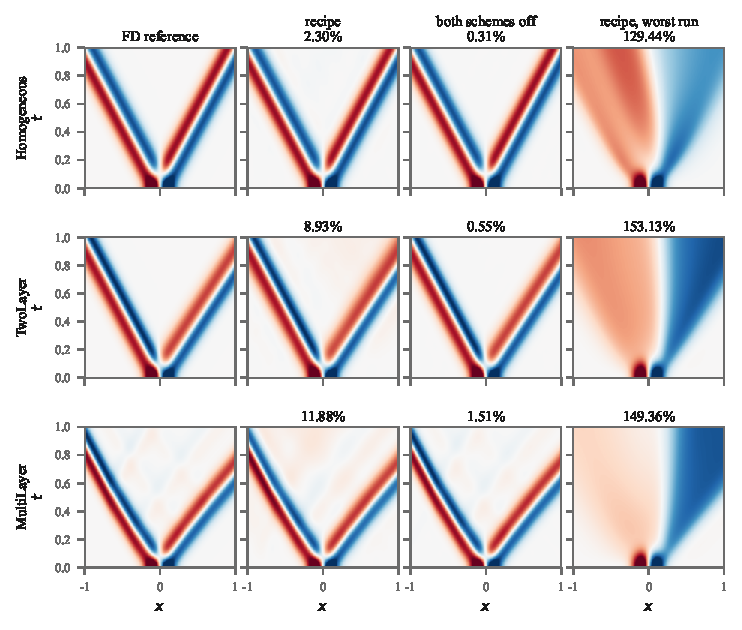
\includegraphics[width=\textwidth]{figures/fig_fields}
\caption{What the error numbers look like. Displacement $u(x,t)$ over the whole
domain, one row per material, on a shared diverging scale set from the
propagating wave. \emph{Column 1:} the finite-difference reference --- the
initial pulse splitting into two counter-propagating waves. \emph{Columns 2--3:}
the same Fourier-feature network under the published recipe and with both
weighting schemes removed; the latter is visually indistinguishable from the
reference. \emph{Column 4:} the recipe's worst run. Note \emph{where} it is
right: the field is correct in a sliver near $t = 0$ and smears into a static
blob after, which is what a causal frontier stuck in its first slab predicts.}
\label{fig:fields}
\end{figure}

\paragraph{How the initial condition is imposed dominates everything else.}
Across the architectures in Table~\ref{tab:pinnmain}, moving the initial
condition from a soft loss term to the hard-constraint ansatz is worth more
than any choice of architecture. Soft-IC runs sit at or above $100\%$ --- the
score of the zero field --- meaning the trained network carries essentially no
signal, while the same architecture with the ansatz reaches single or low
double digits. The IC loss competes with the residual for gradient budget
throughout training, and on this problem it loses; the ansatz removes the
competition by construction.

\paragraph{Even the best network remains behind a classical solve.} Under the
published recipe the
strongest configuration reaches $\PinnRecipeBestErr\%$; the best anywhere in the
sweep, an RBA run, reaches $\PinnRbaBestErr\%$; and the best after the ablation
of Section~\ref{sec:results} reaches $\AblBestErr\%$. The finite-difference
reference reaches $\FDRefErr\%$ in \SI{\FDRefSecs}{\second} on one CPU core, and
the spectral solver goes further still. Figure~\ref{fig:cost}, in
Appendix~\ref{app:supporting}, places both families on the same axes. Nothing about this is specific to a weak baseline:
the classical methods here are textbook schemes, not tuned ones.

\paragraph{The causal frontier almost never leaves the first slabs.}
Of the $\FrontierTotal$ runs that use a causal schedule,
$\FrontierStalled$ end training with at least one slab still weighted at
exactly zero, and $\FrontierOneSlab$ of them never open a second slab at all.
Their median error is $\FrontierStalledMedian\%$. The
$9\,000$-step continuation the runner grants while $w_{\min} < 0.9$ does not
rescue them: it is spent, and the frontier does not move.

Only $\FrontierComplete$ of the $\FrontierTotal$ runs opened all sixteen.
Figure~\ref{fig:causal}
puts a strong stalled run next to the run that advances furthest, so the stall
cannot be dismissed as a generally bad configuration. The latter opens
$\FrontierMaxOpened$ of sixteen slabs. This diagnostic is an association, not
evidence of a mechanism --- the evidence is the ablation below. It nevertheless
sharpens the claim: causal weighting is conditional on the optimiser driving
the early slabs to tolerance, and on this problem that almost never happens.
When it fails to happen, the schedule is far worse than not having used one.

\begin{figure}[t]
\centering

\includegraphics[width=\textwidth]{figures/fig_causal}
\caption{Causal weight $\omega_m$ of each of the 16 time slabs across the Adam
phase, with each panel's final relative $L^2$ in its title. \emph{Left:} the
strongest distinct run whose frontier stalls --- the schedule opens a handful
of slabs and stops, and the rest are weighted at exactly zero for the whole of
training, continuation steps included. \emph{Right:} the run that advances
furthest, opening $\FrontierMaxOpened$ of sixteen slabs.}
\label{fig:causal}
\end{figure}

\paragraph{Both adaptive schemes are costing accuracy.}
% generated by make_tables.py -- do not edit
\begin{table}[t]
\centering
\caption{Switching off the two adaptive weighting schemes, hard-constraint IC. Relative $L^2$ (\%) at the better reported Adam or L-BFGS checkpoint; \emph{causal+GradNorm} is the published recipe and \emph{both off} removes both adaptive schemes.}
\label{tab:ablation}
\small
\begin{tabular}{llrrrr}
\toprule
material & architecture & causal+GradNorm & GradNorm off & causal off & both off \\
\midrule
Homogeneous & VanillaPINN & 129 & 12.9 & 7.37 & \textbf{1.16} \\
 & FourierFeature & 2.30 & 79.3 & 1.000 & \textbf{0.302} \\
 & PirateNet & 105 & -- & \textbf{3.23} & 3.45 \\
 & KAN (spline) & 123 & -- & 437 & \textbf{0.560} \\
 & WavKAN & 24.9 & -- & 21.3 & \textbf{2.70} \\
 & ChebyshevKAN & 37.9 & -- & 6.40 & \textbf{1.62} \\
 & FourierWavKAN & 120 & -- & 2.31 & \textbf{0.624} \\
\midrule
TwoLayer & VanillaPINN & 153 & -- & 6.49 & \textbf{1.42} \\
 & FourierFeature & 8.93 & -- & 1.01 & \textbf{0.554} \\
 & PirateNet & 104 & -- & 6.01 & \textbf{1.14} \\
 & KAN (spline) & 95.9 & -- & 112 & \textbf{0.836} \\
 & WavKAN & 60.2 & -- & 28.7 & \textbf{5.26} \\
 & ChebyshevKAN & 13.2 & -- & 10.4 & \textbf{3.16} \\
 & FourierWavKAN & 18.2 & -- & 4.13 & \textbf{0.923} \\
\midrule
MultiLayer & VanillaPINN & 149 & -- & 19.9 & \textbf{16.2} \\
 & FourierFeature & 11.9 & -- & 2.17 & \textbf{1.51} \\
 & PirateNet & 105 & -- & 4.18 & \textbf{2.76} \\
 & KAN (spline) & 97.2 & -- & 207 & \textbf{5.71} \\
 & WavKAN & 63.9 & -- & 23.0 & \textbf{16.5} \\
 & ChebyshevKAN & 23.0 & -- & \textbf{10.9} & 12.6 \\
 & FourierWavKAN & 13.9 & -- & 7.69 & \textbf{5.55} \\
\bottomrule
\end{tabular}
\end{table}

Table~\ref{tab:ablation} is the main result. Removing \emph{both} schemes ---
pinning $w_{\mathrm{pde}} = w_{\mathrm{bc}} = w_{\mathrm{ic}} = 1$ and
collapsing the causal schedule to a single slab --- wins in
$\AblWins$ of the $\AblPairCount$ architecture--material cells measured against
the published recipe, by
$\AblMinGain$--$\AblMaxGain\times$ with a median of
$\AblMedianGain\times$. The Fourier-feature network goes from
$\PinnRecipeBestErr\%$ under the recipe to $\AblBestErr\%$ without it; the plain
MLP on \emph{TwoLayer} likewise goes from worse than predicting zero to a
single-digit error. Nothing was added to obtain this: same architecture, same
step budget, same optimiser, two adaptive schemes switched off.

The change in the shape of the distribution is as striking as the change in its
best value. Under the recipe, $\PinnRecipeAboveHundred$ of $\PinnRecipeCount$
runs score at or above $100\%$, meaning the trained network carries no more
signal than a zero field. With both schemes off, every cell we have measured
lands well below that threshold. Architectures that looked hopeless under the
recipe become ordinary once the weighting is removed.

The two columns in between separate the causes. Dropping causal weighting alone
accounts for most of the gain in the representative MLP and Fourier-feature
rows. This is consistent with Figure~\ref{fig:causal}: a schedule that leaves
later slabs closed is training on a fraction of the domain, and equal weighting
at least trains all of it. Dropping GradNorm alone is not a uniform fix, but
once causal weighting is gone, removing it helps both representative rows.
Under the full recipe GradNorm can settle with the PDE residual weighted orders
of magnitude below the boundary term.

The causal frontier stalls with GradNorm on \emph{and} off, so the stall is a
property of the schedule on this problem rather than a downstream consequence
of the weighting. Both schemes are behaving exactly as specified; the
specification is what does not suit this problem.

\paragraph{The RBA arm corroborates this independently.}
Table~\ref{tab:pinnvariants} (Appendix~\ref{app:supporting}) reports the SOAP
optimiser, residual-based attention (RBA) in place of causal weighting, and an
L-BFGS-only schedule with no first-order phase. The entry that matters here is RBA, because it is the one
variant that \emph{removes} causal weighting: it replaces the time-slab schedule
with pointwise residual weights and reports $w_{\min} = 1$ by construction. RBA
runs take the top places in the entire sweep, reaching $\PinnRbaBestErr\%$
against the recipe's $\PinnRecipeBestErr\%$ on the same architecture.

That is worth reading carefully, because the natural attribution is wrong. One
would credit the gain to the attention mechanism. The ablation says otherwise:
weighting every time equally, with no attention at all, does better still
($\AblBestErr\%$). On this problem, most of what RBA buys is not what it adds
but what it displaces.

\section{Discussion}
\label{sec:discussion}

We set out to run a control --- a classical baseline on the same problem, same
grid, same metric --- and the control turned into the finding. Two adaptive
schemes that are close to standard equipment in PINN training were, on this
problem, removing an order of magnitude of accuracy while being credited with
producing it.

It is worth being precise about the scope. We are not claiming causal weighting
or GradNorm are bad methods; both were introduced to fix real pathologies and
are reported to do so. We are claiming something narrower and more awkward:
they can silently invert on a problem that looks like the kind they were
designed for, and the published practice of reporting a final error without the
accompanying schedule diagnostics makes that invisible. A causal-training run
computes $w_{\min}$ anyway. If it is pinned at zero, the reported loss is being
evaluated on a fraction of the domain, and the number underneath it means
something different from what it appears to mean.

Why this problem breaks the schedule is not mysterious either. Causal weighting
gates later times behind earlier ones, which is only sound if the earlier times
can actually be driven to tolerance. Here the residual near $t = 0$ is
dominated by a sharp initial pulse ($\sigma_g = 0.1$) whose second derivatives
are large by construction, and the hard-constraint ansatz adds its own
$O(\varepsilon^{-2})$ term there. The first slab never converges, so the gate
never opens.

SOAP provides a useful stress test of that reading: a second-order optimiser is
exactly what one might expect to help on a stiff, badly scaled first slab. It is
nevertheless the highest-variance arm in the sweep, so its results are not a
recommendation. Complementarity between causal weighting and
second-order optimisation remains a hypothesis worth testing at a scale this
study does not have; reporting either without the frontier diagnostic hides
which one is doing the work.

The classical comparison remains the sobering part. Even at $\AblBestErr\%$ the
best network's error is $\AblVsFDRatio\times$ that of a
\SI{\FDRefSecs}{\second}
finite-difference solve and roughly five orders of magnitude behind it in
wall-clock. That is the expected outcome on a 1D forward problem with a known
coefficient field --- the setting where classical discretisation is strongest,
and not the setting PINNs are argued for. The point of running it is that it is
cheap, and it is the only way to notice that a training recipe has gone
backwards.

\paragraph{Limitations.} One seed per configuration and no error bars, so
differences of a few percent between neighbouring configurations should not be
read as real; the order-of-magnitude gaps are. The problem is 1D and forward
only. Training time is reported on a shared GPU whose other tenants we do not
control, so the network timings are upper bounds on a quiet machine, and the
classical timings are single-core CPU --- the comparison is between what each
family costs as it is normally run, not a FLOP-matched one. The hyperparameters
are those specified in the recipe rather than tuned per architecture; a
per-architecture search would likely improve the network numbers, though it
would have to close two orders of magnitude to change the conclusion. Finally,
the causal-stall diagnosis is specific to this initial condition: a smoother
pulse would produce a smaller residual near $t = 0$ and might let the frontier
advance.
